\documentclass[10pt, conference, a4paper, final]{IEEEtran}
\IEEEoverridecommandlockouts
\usepackage{amsmath, amssymb}
\usepackage[margin=1in]{geometry} % Adjust margins if needed
\usepackage{graphicx} % Required for including images
\usepackage{subcaption}
\usepackage{algorithm, algorithmicx} % For algorithms
\usepackage[table,xcdraw]{xcolor} % For colored tables
\usepackage{enumitem} % For better control over list
\usepackage{microtype} % Improves typography
\usepackage{amsmath}
\usepackage{tikz}


\usetikzlibrary{fit}

% Combine graphicx package loading
\usepackage{float}
\usepackage{booktabs} % For professional looking tables

\title{TestifAI: A Comprehensive Testing Framework for Safe AI}
\author{Author Name}
\date{\today}

\begin{document}

\maketitle

\begin{abstract}

    Deep learning (DL) models are critical in high-stakes domains such as autonomous driving, medical diagnostics, and security systems, where their deployment in real-world scenarios requires rigorous robustness testing due to diverse environmental conditions. Traditional metrics like neuron coverage, while essential, do not fully capture all corner cases, which can lead to unexpected model failures. To address this gap, this research introduces a comprehensive testing framework that enhances the correctness evaluation of models through a structured five-stage process. The first stage is specification, defines essential system properties to guide the entire testing process and ensure comprehensive coverage. The second sampling stage, gathering relevant samples for exhaustive model testing. In the test case generation stage, the defined properties are applied to create targeted test scenarios. The testing and probabilistic graph stage validates the effectiveness of these test cases and conducts robustness assessments both locally (within individual category) and globally (across multiple scenarios), employing a Bayesian network for detailed probabilistic and quantitative analysis of performance. The final stage is error summarisation, compiles and analyzes recorded errors to generate actionable graphical error reports and recommendations, thus guiding the refinement of models. This framework not only fills existing gaps in DL testing but also supports the development of models that are correct across varied environmental conditions.
\end{abstract}


\section{Introduction}

% General Problem

% What has been done / citations

% Your more specific problem

% What has been done / what hasn't been done

% Stating your exact problem/objective for the paper

% List the contributions

% Structure of the paper (optional)


Deep neural networks (DNNs) are being more widely used in a variety of applications, yet their correctness in practical applications remains a challenge.

Unlike traditional software, DNNs do not have a clear control-flow structure. They learn their decision policy through training on a large dataset, adjusting parameters gradually using several methods to achieve desired accuracy. Consequently, traditional software testing methods like functional coverage, branch coverage, etc. cannot be applied to DNNs, thereby challenging their use for safety-critical applications. Traditional software testing methods fail when applied to DNNs because the code for DNNs holds no information about the internal decision-making logic.
\begin{itemize}
    \item Input space is extremely large, \textbf{unguided simulation} are highly unlikely to find erroneous behaviour
    \item Standards available in industry but \textbf{lack of logcial structure} and \textbf{system specification}  
     \item Heavily depend on manual collections of test data under different conditions which become expensive as number of test condition increases
     \item  Existing coverage criteria are not detailed enough to notice precise behaviours exhibited by DL systems.
\end{itemize}

% \section{Research Goal}
% This paper aims to develop a systematic framework for evaluating local (in a specific region of the input space) and global (across a broad range of inputs) correctness in deep learning models. 
% The goal is to provide a comprehensive error summary to improve model design and training, ensuring their reliability for real-world applications.

By systematically addressing each aspect from initial specifications to detailed error analysis, we aim to enhance the model's accuracy and reliability in real-world scenarios.


This research makes the following key contributions to the field of deep learning correctness evaluation:
\begin{itemize}
   
    \item We design an \textbf{end-to-end pipeline} for evaluating the correctness of system.
    
    \item We propose a \textbf{conceptual framework} that quantifies both local  and global correctness,with formalized Bayesian probabilistic approach to verify system robustness.
    \item A novel \textbf{error summarization}  approach which allows better identification of model weaknesses related to class and property.

    \item We perform all our \textbf{experiments} using publicly available deep learning models and MNIST dataset.
\end{itemize}

\section{Research Questions}

This paper addresses the following research questions applicable to various vision models and datasets:

\begin{itemize}
    \item How can we design a comprehensive framework to test system correctness?
    \item How can we systematically evaluate the correctness both at local and global levels within framework?
    \item How can error summarization be employed to quantify the impacts on model correctness?
 
\end{itemize}

\section{Background}

AI system is $op(f_1,\dots,f_n)$, where $op$ is some operation.

Specification is...

\section{Approach}
\begin{figure*}{}
    \centering
    % 
\includegraphics[width=\linewidth]{paper_images/frame.pdf}

    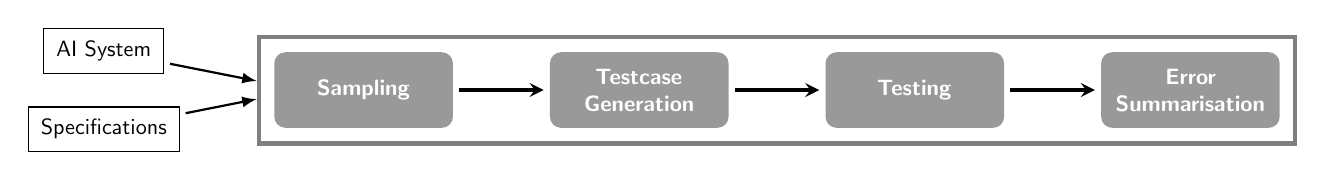
\begin{tikzpicture}[component/.style={fill=gray!80, text=white,
        rounded corners, outer sep=1mm, text width=2.6cm, align=flush
        center, minimum height=1.2cm, scale=0.8},
      input/.style={draw, scale=0.8,  inner sep=2mm, outer sep=1mm}]\sf
      
      \foreach \x/\al/\lab in {%
        1/sampl/Sampling,%
        2/gener/Testcase Generation,%
        3/testing/Testing,%
        4/summary/{Error\\ Summarisation}%
      }{ \node[component] (\al) at (3.5*\x,0) {\textbf{\lab}}; }

      \node[fit=(sampl)(summary), draw=gray, ultra thick] (approach) {};

      \node[input] (aisystem) at (0.2, 0.5) {AI System};
      \node[input] (spec)     at (0.2, -0.5) {Specifications};

      \foreach/\from/\to in {%
        sampl/gener, gener/testing, testing/summary%
      }{ \draw[-stealth, very thick] (\from) -- (\to); }

      \draw[-latex, thick] (aisystem) -- (approach.179);
      \draw[-latex, thick] (spec) -- (approach.181);
    \end{tikzpicture}
    \caption{Overview of Testing Framework}
    \label{fig:graph}
\end{figure*}

This section introduces our comprehensive approach to evaluating an AI system performance, summarised in Figure~\ref{fig:graph}. It takes as input the description of an AI system and a set of relevant specifications. Then it has 4 major components. This step-by-step method highlights the strengths and weaknesses of the model.
\begin{itemize}
% \item The process begins with a detailed description of the properties that need to be tested.

\item We sample inputs for the AI system
\item To thoroughly assess the model, we generate (testcase generation) and test (testing) specific cases based on these properties.
  
\item Following this, we summarise the errors, focusing on how individual image performance (local correctness) translates to the overall system performance (global correctness). 
\end{itemize}


\subsection{Specification}

This step is crucial to specify the deployment environment of the AI system. This allows us to identify and define the relevant properties to ensure correctness in real-world situations. For instance, consider an AI system designed to recognize digits in images, such as in a calculator (sum)  application. The essential properties to verify include:

\begin{itemize}
    \item \textbf{Noise}: Assessing performance under various types of noise (e.g., Gaussian noise, salt-and-pepper noise).
    \item \textbf{Rotation}: Recognizing digits regardless of their orientation.
    \item \textbf{Scaling}: Handling variations in the size of the digits.

    \item \textbf{Occlusion}: Maintaining recognition accuracy with partially occluded digits.

\end{itemize}

Let \( I \) represent the input image and \( \hat{I} \) the transformed image subjected to various conditions. The transformations can be modeled as follows:

\begin{align}
    \hat{I}_{noise} &= I + N \\
    \hat{I}_{rotation} &= R(\theta) \cdot I \\
    \hat{I}_{brightness} &= B(b) \cdot I \\
    \hat{I}_{scaling} &= S(s) \cdot I \\
    \hat{I}_{occlusion} &= I \cdot O 
\end{align}

Where:
\begin{itemize}
    \item \( N \) represents the noise added to the image.
    \item \( R(\theta) \) denotes a rotation matrix with angle \( \theta \).
    \item \( B(b) \) denotes brightness with factor \( b \).
    \item \( S(s) \) is a scaling matrix with scale factor \( s \).
    \item \( O \) is an occlusion mask.
\end{itemize}

The performance of the AI system is evaluated based on its ability to correctly recognize the digit in \( \hat{I} \) for each transformation.



\subsection{Sampling}
 The sample selection process involves a random but balanced choice of samples from each class, focusing exclusively on instances that the model has correctly predicted. This method ensures a representative and fair distribution of data across all classes.

\begin{itemize}

    
        \item Model Utilization:
            \begin{itemize}
                \item A pre-trained CNN model is utilized to select samples.
                \item Let \( X = \{x_1, x_2, \dots, x_N\} \) denote the set of MNIST images. The model function \( f \) predicts:
                \[ f(x_i) \rightarrow y_i \]
                \item The filter function \( g \) identifies accurate predictions, defined as:
                \[ g(x_i) = 
                \begin{cases} 
                1 & \text{if } f(x_i) = \text{true label of } x_i \\
                0 & \text{otherwise}
                \end{cases} \]
                \item The subset \( S \) includes only correctly predicted images:
                \[ S = \{x_i \in X \mid g(x_i) = 1\} \]
            \end{itemize}
        \item Random Selection of Samples:
            \begin{itemize}
                \item Randomly selects 100 samples from each class in \( S \), totaling 1000 samples.
                \item The random selection function \( R \) is defined to ensure:
                \[ R(S_c, 100) \text{ for each class } c \text{ in } S \]
                where \( S_c \) represents the samples of class \( c \) within \( S \).
            \end{itemize}

\end{itemize}


\subsection{Test Case Generation}

This section outlines the generation of test cases to assess model robustness through properties such as noise, rotation, brightness adjustments, occlusion, and scaling.

\begin{itemize}
    \item \textbf{Noise Addition:} Noise is added to an image \( x_i \) using a Gaussian noise model. The noise function \( p_n \) is defined as:
    \[ p_n(x_i, \sigma) = x_i + \epsilon \]
    where \( \epsilon \sim \mathcal{N}(0, \sigma) \) denotes the Gaussian noise with mean zero and standard deviation \(\sigma\).

    \item \textbf{Rotation:} The rotation of an image \( x_i \) by an angle \(\theta\) is modeled by the rotation function \( p_r \):
    \[ p_r(x_i, \theta) = \text{rotate}(x_i, \theta) \]
    where \(\text{rotate}(\cdot, \theta)\) represents the rotation operation.

    \item \textbf{Brightness Adjustment:} Brightness adjustment of an image \( x_i \) is controlled by a multiplicative factor \( \beta \), which scales the intensity of all pixels. The brightness function \( p_b \) can be defined as:
    \[ p_b(x_i, \beta) = \beta \cdot x_i \]
    where \( \beta > 1 \) increases brightness, and \( \beta < 1 \) decreases it. This approach ensures that the image's contrast is preserved while adjusting its brightness.

    \item \textbf{Occlusion:} Occlusion is simulated by covering parts of the image \( x_i \) with a mask \( M \). The occlusion function \( p_o \) is defined as:
    \[ p_o(x_i, M) = x_i \cdot M \]
    where \( M \) is a binary mask that obscures parts of the image, with \( M = 0 \) for occluded pixels and \( M = 1 \) for visible pixels.

    \item \textbf{Scaling:} Scaling of an image \( x_i \) is controlled by a scaling factor \( s \), which resizes the image. The scaling function \( p_s \) is defined as:
    \[ p_s(x_i, s) = \text{scale}(x_i, s) \]
    where \(\text{scale}(\cdot, s)\) represents the scaling operation, resizing the image by a factor of \( s \).
\end{itemize}


\subsection{Testing }

The Testing section evaluates how accurately and confidently the  AI subsystem's predicts under various properties applied to images from each class. This phase focuses on directly measuring and quantifying the correctness of the  AI subsystem's.

 After generating test cases, measure the  AI subsystem's confidence for each class under each type of property.
     

  
    \subsubsection{Local Correctness}

    Local correctness involves checking the AI subsystem's performance on individual images subjected to different transformations. For each image \( x \) from a set of samples \( X \), the AI subsystem produces a confidence score \( f(x) \) representing its certainty in recognizing the digit. The local correctness for a transformation \( T \) applied to an image \( x \) is defined as:

    \[
        \text{Local Correctness}(x, T) = f(T(x))
    \]

    Where \( T \) can be any transformation such as noise addition, rotation, brightness adjustment, occlusion, or scaling. Each transformation is evaluated to determine its impact on the confidence score.

    
    \subsubsection{Global Correctness}

    Global correctness evaluates the AI subsystem's performance on combinations of images and transformations, such as adding two digits under different transformations. Given a set of 100 samples for each digit (0-9), we randomly select images to form digit pairs. The global correctness assesses the combined confidence for recognizing the result of operations like addition under each transformation.

    For each transformation \( T \), we define local correctness for digits \( d_1 \) and \( d_2 \) as follows:
    
    \[
    \text{LC}_{T}(d_1) = \text{Local Correctness}(x_1, T)
    \]
    \[
    \text{LC}_{T}(d_2) = \text{Local Correctness}(x_2, T)
    \]
    
    Where \( x_1 \) and \( x_2 \) are randomly selected images representing digits \( d_1 \) and \( d_2 \).
    
    The global correctness for each transformation is then defined as the product of the local correctness values:
    
    \[
    \text{GC}_{T} = \text{LC}_{T}(d_1) \times \text{LC}_{T}(d_2)
    \]
    
    To determine the optimistic and pessimistic global correctness across all transformations, we calculate the following:
    
    \begin{itemize}
        \item \textbf{Optimistic Global Correctness}:
        \[
        \text{GC}_{opt} = \max_{T} (\text{GC}_{T})
        \]
        \item \textbf{Pessimistic Global Correctness}:
        \[
        \text{GC}_{pes} = \min_{T} (\text{GC}_{T})
        \]
    \end{itemize}
    
    For the addition operation, if we denote the sum of digits \( d_1 \) and \( d_2 \) as \( d_{\text{sum}} \), the overall global correctness for the operation is:
    
    \[
    \text{Overall Global Correctness} = \min(\text{GC}_{opt}, \text{GC}_{pes})
    \]
    
    Where each transformation is evaluated separately, and the global correctness is determined based on the individual probabilities of correct recognition for each digit under each transformation.
    \begin{figure}{}
        \centering
        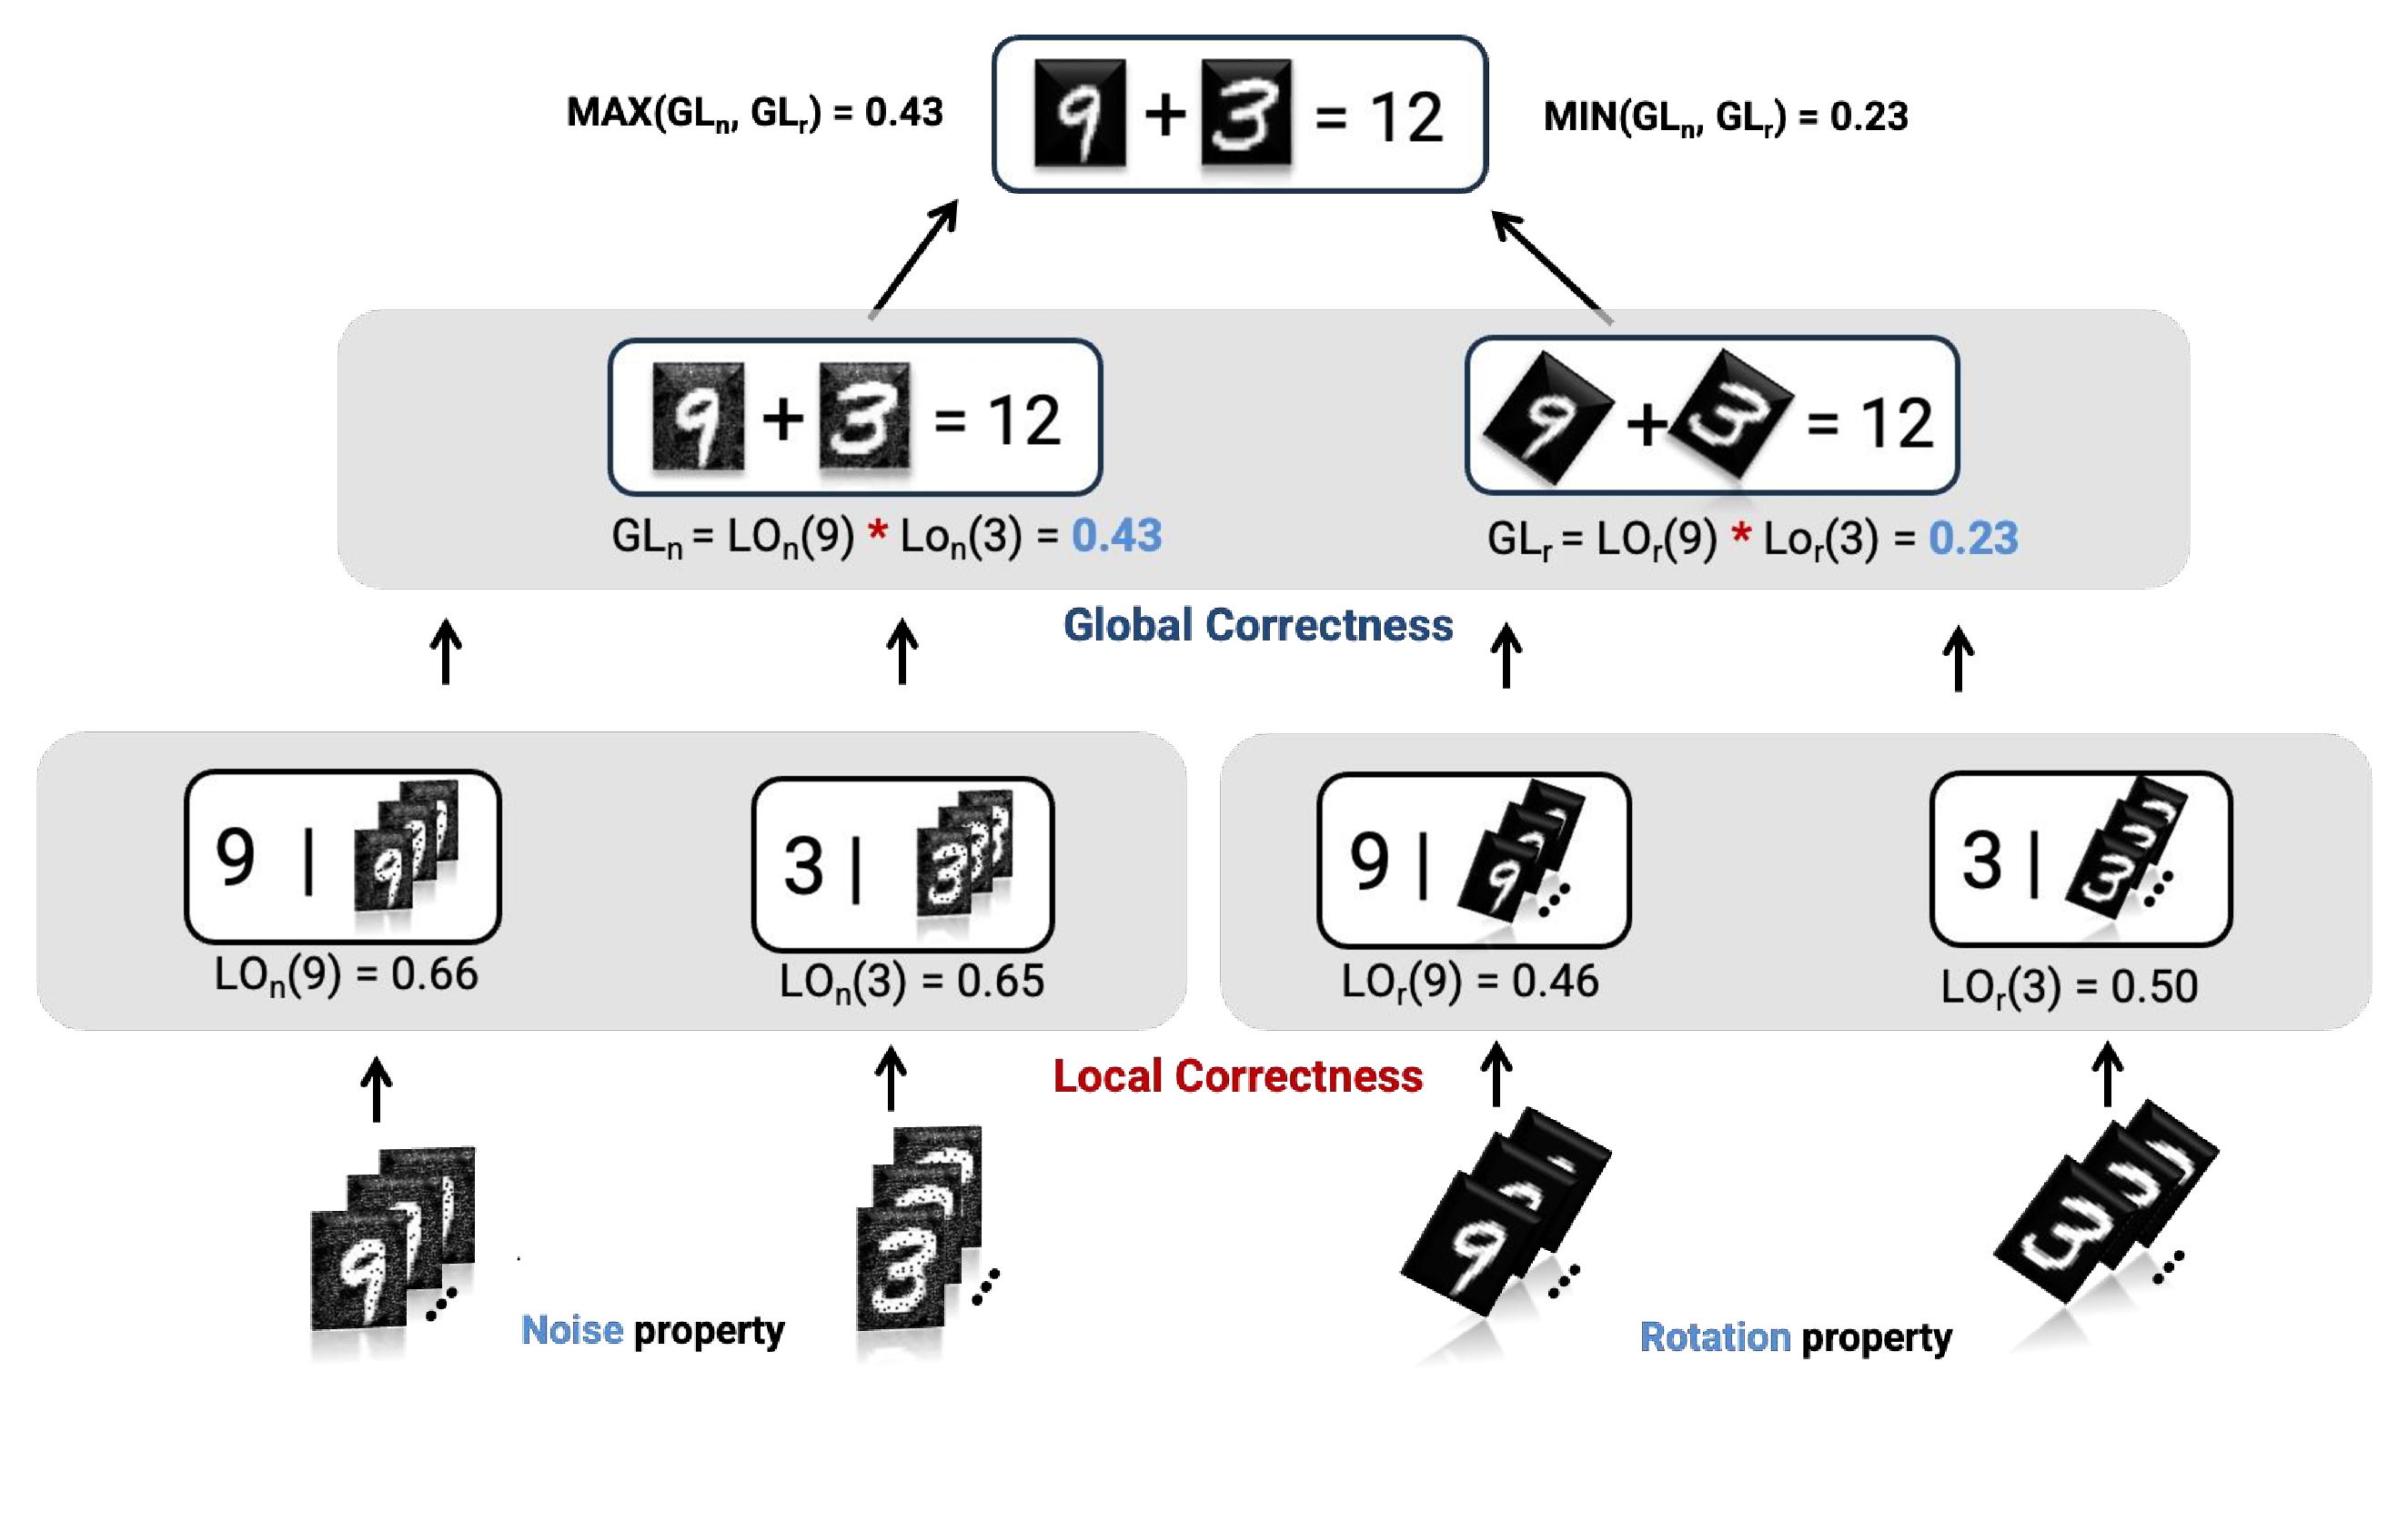
\includegraphics[width=\linewidth]{paper_images/noise_rotation_localcal_global.pdf}
        \caption{Graphical View of Local and Global Correctness}
        \label{fig:graph}
    \end{figure}

 
\subsubsection{how to write bayesian story, either it would be proper section or adust each baesian equation in all steps??? }
\subsection{Error Summarization}

\begin{figure}[H]
    \centering
    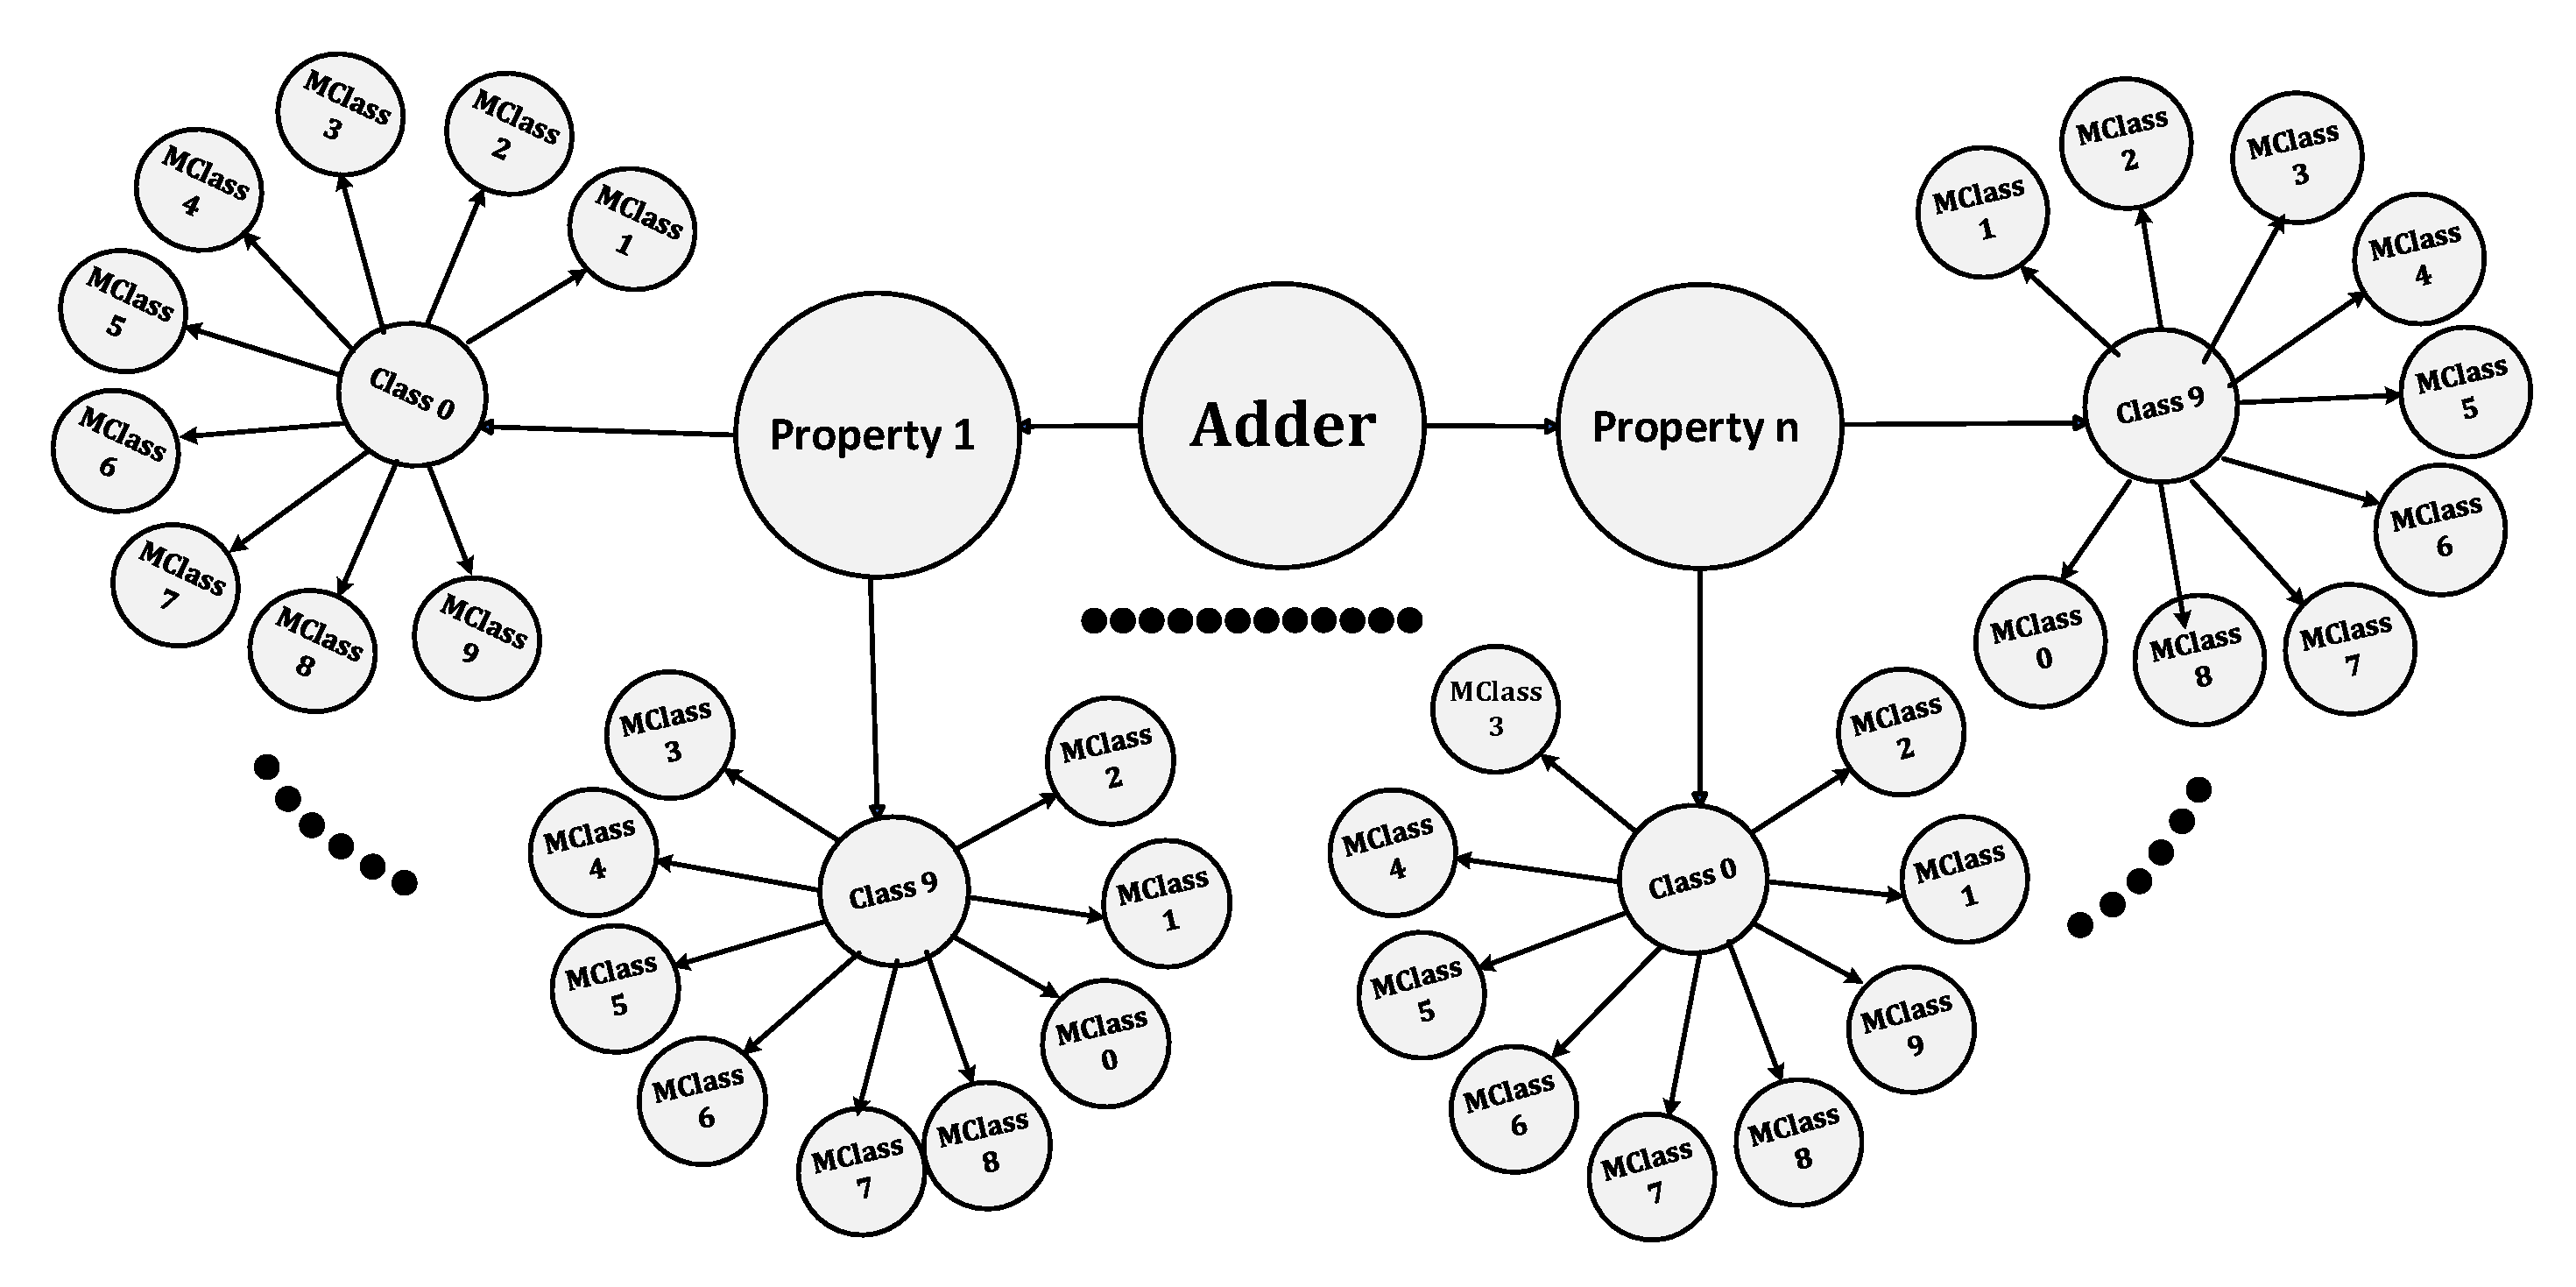
\includegraphics[width=\linewidth]{paper_images/step5.pdf}
    \caption{Diagram of Error Summarization Highlighting Class-Property Impact}
    \label{fig:error-summarization}
\end{figure}





\section{Experiments}


\section{Threats to Validity}

This section outlines significant limitations and assumptions in our study that may affect the validity and reliability of our findings.

\begin{itemize}
    \item \textbf{Random Sampling:} Our current approach assumes a uniform distribution of samples across all classes, which may not represent the true complexity and variability within real-world data. This uniform sampling can lead to biased evaluations if the class distribution in practical applications is skewed or non-uniform. We plan to enhance our sampling techniques to better capture the diversity and distribution of data in realistic scenarios. Improved sampling strategies will help in developing more robust and generalizable error summarization methods.
\end{itemize}


\section{Related Work}
% Your content here

\section{Conclusion}
% Your conclusion here

\begin{thebibliography}{01}
    \bibitem{Saad} Reference details
\end{thebibliography}

\end{document}
